%!TEX root = main.tex
\chapter[Evaluaci\'on]{Evaluaci\'on}
\label{sec:evaluation}

En la secci\'on \ref{sec:intro.objetivos} definimos las motivaciones y objetivos de esta tesis, donde el principal consta del dise\~no y desarrollo de un operador de mutaci\'on, altamente configurable, para expresiones encadenadas. Luego, en la secci\'on \ref{sec:preliminares.mutation.opevaluation} definimos que propiedades afectan el an\'alisis de \emph{mutation testing}, cantidad de mutantes, mutantes equivalentes, dificultad de detecci\'on, acoplamiento con fallas reales, y redundancia de mutantes (o acoplamiento entre mutantes). En este capitulo realizamos la evaluaci\'on de nuestro ``meta-operador'', \emph{prvo}, para determinar la utilidad pr\'actica de la misma.

\section{Configuraci\'on}
\label{sec:evaluation.prvoconfig}

Antes de evaluar a \emph{prvo}, es necesario que definamos una configuraci\'on particular para el mismo. Teniendo en cuenta que la configuraci\'on sobre miembros de clases a utilizar o evitar, es decir, una de las propiedades principales que regula el conjunto de expresiones a utilizar durante la mutaci\'on, es algo que debe definirse por cada proyecto, vamos entonces para este caso, a definir de manera general que criterio vamos a utilizar para configurar esta propiedad para cada proyecto. El primer problema a resolver para poder definir esta configuraci\'on y el criterio para expresiones a utilizar, es especificar que tipo de fallas estamos interesados en representar, puesto que lo mejor no es una configuraci\'on que permita representar m\'ultiples fallas sino una que se centre en un tipo de falla espec\'ifica. De acuerdo a nuestro ejemplo motivador, dado en la secci\'on \ref{sec:intro.objetivos}, el tipo de fallas que queremos representar son aquellas que involucran expresiones de navegaci\'on, es decir, expresiones encadenadas de tama\~no al menos 1, y que resultan de el acceso al miembro incorrecto de una clase. Estas fallas no parecen estar de acuerdo con el ejemplo, recordemos que \'este utiliza un m\'etodo \emph{dequeue()} que solo tiene una l\'inea donde reasigna el valor a un puntero, y la falla est\'a en la falta de c\'odigo, como controles y reasignaci\'on de otros punteros, sin embargo, modificar un miembro en las expresiones halladas en la \'unica sentencia del m\'etodo, genera la necesidad de mejorar el test suite. Por parte de las fallas mencionadas como no acopladas actualmente a fallas reales, descriptas en \ref{sec:prvo.prvoTargetedFaults}, dentro de estas vamos a estar representando a:

\begin{enumerate}[label=\arabic*), leftmargin=.75cm,align=left]
	\item Llamada a un m\'etodo similar de la misma librer\'ia
	\item Acceso directo a un campo\footnote{Solo para campos de las clases bajo evaluaci\'on}
\end{enumerate}

%TODO: SEGUIR ACA

\section{Evaluaci\'on}

El objetivo de la evaluaci\'on es analizar si \emph{prvo}, como familia de operadores de mutaci\'on para expresiones encadenadas, es de hecho una contribuci\'on a \emph{mutation testing}. La contribuci\'on te\'orica de nuestra familia de operadores queda clara en nuestras motivaciones y el dise\~no de \emph{prvo}:
\begin{quote}
  Existen fallas reales relacionadas a expresiones encadenadas que no son representadas por mutantes generados por operadores de mutaci\'on existentes.
\end{quote}
Sin embargo, la contribuci\'on en la pr\'actica puede no existir, \emph{las fallas que representa prvo est\'an subsumidas por aquellas que representan operadores existentes}; \emph{las mutaciones generadas por prvo son triviales de detectar, o son equivalentes}; \emph{la cantidad de mutantes generados por prvo excede los potenciales beneficios de su uso}. Es por esto que nuestra evaluaci\'on se centra en las siguientes preguntas:
\begin{itemize}
	\item \textbf{RQ1} El uso de \emph{prvo} complementa de manera significativa a los operadores de mutaci\'on tradicionales?
	
	\item \textbf{RQ2} Cual es el costo adicional de utilizar \emph{prvo}, en mutation testing?
\end{itemize}

La motivaci\'on para \textbf{RQ1} est\'a basada en que un nuevo operadores no ser\'ia \'util si fuera redundante con respecto a los existentes. Para responder \textbf{RQ1} vamos a utilizar \emph{dynamic mutant subsumption}. Este an\'alisis permite, para un programa particular y un conjunto de tests particulares, evaluar que mutantes resultan indispensables y cuales son redundantes para la evaluaci\'on del conjunto de tests. Vamos a utilizar principalmente como benchmark, implementaciones de estructuras de datos orientadas a objetos, en \emph{Java}. La raz\'on para considerar un benchmark as\'i, es que este tipo de implementaciones hace un uso substancial de expresiones de navegaci\'on, incluyendo tipos recursivos de datos. Nuestro benchmark va a estar compuesto entonces mayormente por implementaciones de collecciones:  \emph{Apache's TreeList}, una implementaci\'on de listas utilizando \'arboles; \emph{Apache's NodeCachingList}, una lista encadenada con una cach\'e de nodos; \emph{AvlTree}, una implementaci\'on cl\'asica de \'arboles balanceados; \emph{BinomialHeap}, una implementaci\'on basada en referencias de mont\'iculos; y \emph{TreeSet}, una implementaci\'on de conjuntos utilizando \'arboles red-black. %TODO: AGREGAR CASOS

Para responder a \textbf{RQ1} vamos a utilizar mutation score, toughness (cuantos tests un mutante sobrevive antes de ser detectado), y dynamic mutant subsumption para detectar mutantes dominadores. Adem\'as se van a analizar los mutantes no detectados para detectar aquellos que son equivalentes, esto solo se va a realizar para aquellos generados por \emph{prvo}. A su vez, si bien en principio evaluar cuantos nodos dominadores involucran a \emph{prvo} parece una buena m\'edida, es importante destacar que un nodo puede contener varios mutantes equivalentes entre s\'i, entonces utilizar directamente la relaci\'on \texttt{(nodos dominadores que involucran a prvo)/total de nodos dominadores}, no sirve de mucho por que la informaci\'on obtenida no va a necesariamente reflejar cuanto domina \emph{prvo} sobre todos los mutantes. Por esto, vamos a utilizar el concepto de nodos puros descripto previamente en \ref{sec:implementation.dynamicSubsumption.dominators} para poder medir la relaci\'on de nodos puros dominadores de \emph{prvo}.

Vamos a necesitar proveer conjuntos de tests para realizar nuestra evaluaci\'on. Sobre todo, para que nuestro an\'alisis sea significativo, necesitar\'iamos utilizar conjuntos de tests relativamente ``buenos'', dado que si fu\'eramos a utilizar test suites pobres (con baja cobertura de c\'odigo por ejemplo), podr\'iamos no obtener relaciones entre el uso o no de \emph{prvo}, o resultados que solo se mantienen al usar tests de mala calidad.

Dynamic mutant subsumption es un an\'alisis que se ve beneficiado por tener gran cantidad de tests. Entonces es necesario establecer como vamos a generar nuestros tests. Manualmente, tiene la ventaja de hacer tests teniendo un conocimiento de no solo la sem\'antica del programa bajo prueba, sin\'o un tambi\'en de la sint\'axis. Las desventajas vienen por dos lados, por uno, generar manualmente una gran cantidad de tests, representa un trabajo complejo y tedioso; por el otro lado, no es posible garantizar imparcialidad, incluso de manera subconsciente uno podr\'ia caer en la tentaci\'on de escribir tests sabiendo el impacto que los mismos van a tener en la evaluaci\'on de \emph{prvo}. Autom\'aticamente, tiene la ventaja de que permite generar una gran cantidad de tests, tan grande como uno quiera para algunas herramientas, y brinda imparcialidad. Al mismo tiempo, utilizar herramientas autom\'aticas permite generar varios test suites distintos con la misma ``calidad'', lo cual nos sirve para poder repetir los experimentos y eliminar, al menos en cierto grado, la incertidumbre de si nuestros resultados son buenos por que usamos un conjunto de tests particularmente favorable para nosotros. 

Dentro de las herramientas de generaci\'on autom\'atica de tests, creemos que \emph{Evosuite} y \emph{Randoop} son dos de las mejores en la actualidad, al menos para \emph{Java}. Evosuite utiliza algor\'itmos gen\'eticos para, a partir de un conjunto inicial de test suites, hacer evolucionar a estos hasta lograr el ``mejor''. Si bien Evosuite suele generar buenos tests, el inconveniente para nuestro estudio es que \'estos son relativamente pocos, incluso si se incrementan los recursos disponibles para la herramienta, lo \'unico que se mejora son la calidad de los tests generados (con respecto a uno o varios criterios de evaluaci\'on), pero como dijimos, necesitamos conjuntos grandes de tests. Es por esto que creemos que complementar los tests de Evosuite con los generados por Randoop, una herramienta que genera tests mediante aleatoriedad en donde la cantidad de tests generados se puede controlar con los recursos utilizados, es la mejor forma para generar los test suites que vamos a utilizar para evaluar \emph{prvo}.

Nuestro an\'alisis tienen que tener en cuenta a \emph{prvo} como un operador adicional\footnote{La familia de operadores de \emph{prvo} la consideremos como un solo operador.}. Los otros operadores de mutaci\'on, con los que vamos a comparar, son aquellos considerados en el conjunto de operadores de mutaci\'on suficientes \cite{bibliography.mutation.selection.Offutt96, bibliography.mutation.selection.ASN2008} e implementados en \emph{mu$Java$}. Detalles de todos los operadores a nivel de m\'etodo soportados por \emph{mu$Java$} y subsecuentemente por \emph{mu$Java$++} pueden encontrarse en \cite{muJavaMOPS}. 

Si bien cuando mencionamos las propiedades a tener en cuenta en el dise\~no de operadores de mutaci\'on, vimos que la mayor\'ia de las mismas tienen un gran impacto en el significado del mutation score obtenido, \'este sigue siendo un valor com\'unmente utilizado en estudios, y representa \textbf{el} indicador asociado a \emph{mutation testing}. Por lo tanto nos interesa observar como \'este es afectado por la inclusi\'on de \emph{prvo}. Teniendo en cuenta que, una suba en el mismo representar\'ia el hecho de que \emph{prvo} gener\'o mutantes que en su mayor\'ia fueron detectados; mientras que una baja, representar\'ia que \emph{prvo} gener\'o mutantes que representan nuevas fallas no detectadas por el test suite. Es necesario aclarar, que en cualquier caso, no es posible sacar conclusiones solamente basados en estos cambios, por eso analizamos equivalencia y dominancia.

Tal como describimos en la secci\'on \ref{sec:implementation.dynamicSubsumption.dominators}, nuestro an\'alis va a utilizar informaci\'on obtenida de los grafos de \emph{dynamic mutant subsumption}, particularmente como cambia la representaci\'on de los operadores en los nodos dominantes, con y sin \emph{prvo}. La pureza de los nodos nos va a ser de gran utilidad en este an\'alis para poder eliminar los casos en donde mutantes generados por distintos operadores tienen gran presencia en los nodos dominantes, pero son equivalentes entre s\'i.

Para poder evitar casos donde el test suite utilizado es particularmente beneficioso o desfavorable para \emph{prvo}, vamos a realizar m\'ultiples experimentos para el mismo programa con distintos test suites generados de manera autom\'atica. Dado que las herramientas utilizadas tienen ambas distintos grados de aleatoriedad, vamos a utilizar un conjunto fijo de ``semillas'' para garantizar cierto grado de replicaci\'on. Incluso con la misma semilla, al ser herramientas que se ejecutan con un presupuesto de tiempo determinado, la cantidad de operaciones que logran realizar bajo \'este, no siempre es la misma, generando no determinismo. Creemos que la repetici\'on de nuestros experimentos es suficiente para contrarrestar los efectos del mismo.

Respecto a \textbf{RQ2}, el foco est\'a en la eficiencia; incluso si \emph{prvo} (o cualquier operador) resulta ser \'util en cuanto a los mutantes que genera, su uso se vuelve prohibitivo si los costos asociados a su utilizaci\'on son muy altos. Este costo est\'a t\'ipicamente asociado a dos factores: la complejidad en la generaci\'on de los mutantes, y el n\'umero de mutantes generados. El primero es com\'unmente ignorada, dado que salvo casos muy raro, los recursos utilizados son usualmente despreciables. El segundo factor es en general el que representa la preocupaci\'on principal para el dise\~no de un operador de mutaci\'on, dado que en el peor caso, todos los tests deben ser ejecutados para todos los mutantes al computar el \emph{mutation score}. Es por eso que cuantos mutantes genera \emph{prvo} es la m\'etrica principal para analizar su costo.

%Due to space restrictions, we only report here a summary of the experimental results. Further information, along with a replication package, can be found in:
%\begin{center}
%	\texttt{https://sites.google.com/view/prvo/}
%\end{center}

\section{Resultados experimentales}

En esta secci\'on vamos a discutir los resultados de nuestra evaluaci\'on, enfoc\'andonos primero en \textbf{RQ1}. La figura \ref{subsumption-results} resume los resultados de nuestro an\'alisis de subsuma. Los resultados se muestran por caso de estudio. Cada gr\'afico incluye el porcentaje de mutantes dominantes por operador de mutaci\'on, usando la media de todas las repeticiones para el mismo caso de estudio. \'Estas representan los experimentos, que como anteriormente explicado, incluyen una ejecuci\'on usando \emph{prvo} y una sin usarlo.

Let us now discuss the results of our evaluation, focusing first on \textbf{RQ1}. Figure~\ref{subsumption-results} summarizes the results of our subsumption analysis. Results are shown per case study. Each chart includes the percentage of dominator mutants per mutation operator, using the median of all runs for the same case study. These were run, as explained earlier in this section, twice; first, without considering \emph{prvo}, only considering existing mutation operators. Results are shown in green bars. For instance, for Apache's TreeList, over 35\% of the LOI (Logical Operator Insertion) mutants were dominators, in the runs where \emph{prvo} was not considered. Obviously, there are no green bars for the PRVO column. When \emph{prvo} is taken into account, and experiments re-run, these percentages change. Percentages of dominator mutants per operator, in runs where \emph{prvo} was taken into account, are shown as red bars in the charts (again, with the median of all experiments for the same case study). For instance, for Apache's TreeList, the percentage of LOI mutants that are dominators is decreased to less than 30\% when \emph{prvo} is considered. Also, for this same case study, the percentage of dominator mutants associated with \emph{prvo} is 25\%. 

There is one last piece of information highlighted in Figure~\ref{subsumption-results}. Recall that, when building subsumption graphs to perform dynamic subsumption analysis, all mutants that dominate each other are ``collapsed'' as a single node. Thus, if such a node is ``dominator'' in the graph, all mutation operators that contributed mutants to the set are considered dominators. For the case of \emph{prvo}, we would like to know which dominator nodes are \emph{only} composed of \emph{prvo} mutants. We show that information in the charts with a blue bar. For instance, for Apache's TreeList, over 20\% of the dominator mutants in the runs where \emph{prvo} was considered were ``pure'' \emph{prvo}, i.e., they were not accompanied as subsumers by mutants other than \emph{prvo} ones. 

Let us now analyze these results. The most important observation is that in almost all case studies (with the exception of Apache's NodeCachingList), \emph{prvo} is among the top operators in terms of dominance. Indeed, \emph{prvo} is in general one of the top three dominator operators, accompanying typical ``sufficient'' mutators, such as ROR (Relational Operator Replacement, LOI, or the family of Arithmetic Operator Insertion operators (AOIS, AOIU, AOIB, \dots). Also, it is important to remark that, in the presence of \emph{prvo}, the dominance of other operators is in general decreased, as their dominance over some nodes is ``transferred'' towards \emph{prvo}. More precisely, \emph{prvo} ``dominates'' some ``root'' mutants, i.e., mutants that in the absence of \emph{prvo} are dominators.    

Clearly, our experimental results support a positive answer to \textbf{RQ1}, i.e., \emph{prvo} does in fact significantly complement traditional mutation operators; it generally produces a large set of mutants not dominated by existing operators, and exhibits a high number of dominant mutants, that may even allow us, at least in the context of our experiments, to consider \emph{prvo} a sufficient operator (along with the traditional sufficient ones). 

\begin{figure}[t]
	\begin{center}
		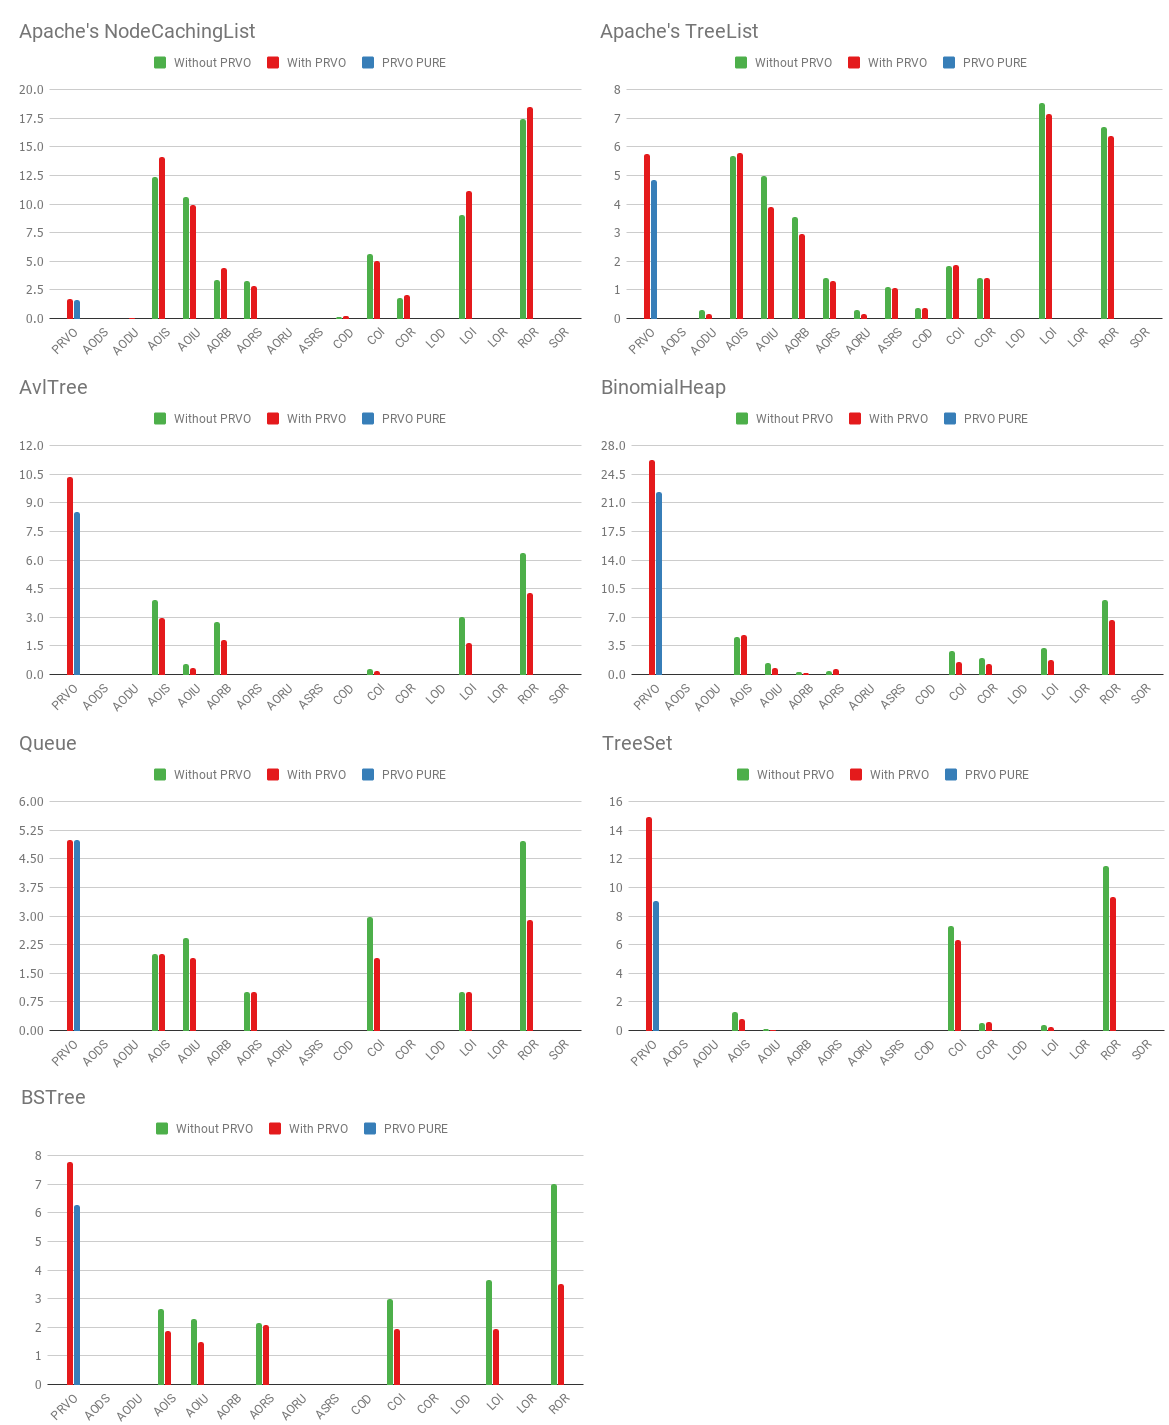
\includegraphics[width=12cm]{figures/Tables.png}
	\end{center}
	\caption{Summary of dynamic subsumption analysis}
	\label{subsumption-results}
\end{figure}

Now let us turn our attention to \textbf{RQ2}. Figure~\ref{mutants-results} summarizes the results for mutants generation, comparing the number of mutants obtained when \emph{prvo} is disabled (green bars) with those for the cases in which \emph{prvo} is enabled (blue bars). We also report in this summary the number of equivalent \emph{prvo} mutants (i.e., mutants that are semantically equivalent to the original program, and thus cannot be killed no matter which tests we consider) produced for each case study.

For the majority of the case studies, the number of mutants that \emph{prvo} generates is a small ``overhead'' over the set of mutants generated when \emph{prvo} is disregarded. TreeSet and BinomialHeap are two exceptions, where \emph{prvo} alone generates roughly the same number of mutants as all the other operators together. The reason is that these case studies feature methods with a high number of navigational expressions in conditions and other comparisons, of the kind \texttt{expr == null}. These expressions admit a single ROR mutation (replacing equals by not equals), whereas \emph{prvo} produces many more mutations from the same mutation point. Notice however that in these two case studies, \emph{prvo} is a clear dominator (see Figure~\ref{subsumption-results}); in particular, it is noticeable how the dominance of other operators is significantly diminished when \emph{prvo} is taken into account. Our preliminary answer to \textbf{RQ2} is then that the added cost associated with \emph{prvo} is in general low, although there are cases where the number of \emph{prvo} mutations may explode. These cases show, in our experiment, a greater dominance of \emph{prvo} over other mutations, suggesting that there is margin for optimization via test/mutant prioritization in these cases. Still, these results call for refinements to \emph{prvo}, that may lead to a consistently low overhead in mutation analysis, with respect to traditional mutations.

Regarding equivalent mutants, the results are interesting too. A very low number of mutants were equivalent to the original program. Notice that this is an important number. When an operator produces many equivalent mutants, the corresponding mutation scores are artificially (and misleadingly) reduced, since having mutants that cannot be killed will make scores to tend towards lower number. Having small numbers of such mutants is then clearly a good sign.     



\begin{figure}[t]
	\begin{center}
		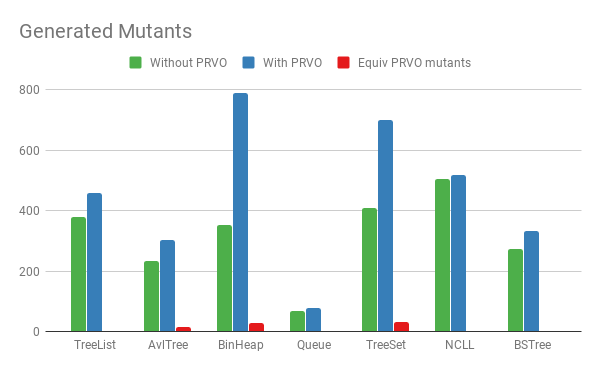
\includegraphics[width=9cm]{figures/Generated_Mutants.png}
	\end{center}
	\caption{Summary of mutants generated.}
	\label{mutants-results}
\end{figure}


\section{Amenazas a la validez}

Nuestra evaluaci\'on experimental est\'a limitada a implementaciones relativamente peque\~nas de colecciones en \emph{Java}. Las razones por las que seleccionamos estas implementaciones como casos de estudio fueron parcialmente descriptas anteriormente, y esencialmente tiene que ver con que estos proyectos son buenos representantes de implementaciones orientadas a objetos con usos sofisticados de expresiones de navegaci\'on (por ejemplo, utilizan tipos de datos recursivos, y m\'ultiples referencias a objetos distintos del mismo tipo). Otra raz\'on por la que nos limitamos a estos casos de estudio tiene que ver con el alto costo de an\'alisis de mutaci\'on. Especialmente en nuestro contexto, en donde las caracter\'isticas de nuestra evaluaci\'on nos lleva a la necesidad de realizar numerosos an\'alisis de mutaci\'on, en particular, computar los grafos de subsuma de mutantes har\'ia inviable esta evaluaci\'on si fu\'eramos a utilizar proyectos m\'as grandes.

Nuestro an\'alisis est\'a tambi\'en atado a una forma espec\'ifica de generar tests, \'esta se basa en el uso de dos herramientas particulares, Evosuite y Randoop espec\'ificamente. \'Esto est\'a motivado por el tipo de test suites que resultan de relevancia para an\'alisis de subsuma. Dado el impacto que tiene el presupuesto de tiempo que se brinda a las herramientas que utilizamos para generar los test suites, nuestros resultados podr\'ian estar siendo afectados por el mismo. Para contrarrestar esta potencial amenaza, corrimos los experimentos con distintos presupuestos de tiempo, lo que llev\'o a test suites de distintos tama\~nos, y por supuesto resultados diferentes. Sin embargo \'estos son consistentes, es decir, las observaciones para un experimento mantienen la misma tendencia para todos los presupuestos de tiempo utilizados.

Gran parte de nuestra evaluaci\'on experimental es m\'as bien objetiva, por ejemplo, la noci\'on de subsuma, y est\'an calculadas por nuestra implementaci\'on. Hicimos nuestro mejor esfuerzo para garantizar la validez de nuestros resultados, pero a\'un as\'i nuestra implementaci\'on podr\'ia contener defectos que afecten a nuestros resultados. La equivalencia de programas, requerida para analizar mutantes equivalentes, es un problema indecidible. Varias t\'ecnicas han sido propuestas para resolver este problema (obviamente de manera aproximada), sin embargo, la verificaci\'on manual sigue siendo una de las m\'as utilizada en la pr\'actica, y es la que hemos utilizados nosotros. Afortunadamente este an\'alisis estuvo limitado a un n\'umero muy peque\~no de mutantes y cualquier duda sobre la equivalencia de uno, fue siempre anotada en desventaja de \emph{prvo}, es decir, ante la duda, se consider\'o el mutante como equivalente. Creemos que los errores que podemos haber cometido con respecto a equivalencia de mutantes, no afectan de manera significativa nuestras conclusiones.

Nuestro an\'alisis est\'a tambi\'en limitado a un conjunto arbitrario de operadores de mutaci\'on. Podr\'iamos haber considerado otros operadores, por ejemplo los que act\'uan a nivel de clases (en contraposici\'on de los que usamos que act\'uan a nivel de m\'etodos) \cite{bibliography.mutation.class-level-ops}. \'Estos, est\'an relacionados a nuestro trabajo, en el sentido de que se aplican a programas orientados a objetos, pero se enfocan en aspectos ortogonales como visibilidad (cambiando la visibilidad de m\'etodos y campos en una clase). Decidimos concentrarnos en los operadores que se consideran tradicionales, en el contexto de mutation testing, y creemos que hemos tenido en cuenta a los m\'as significativos, basado en los que est\'an disponibles en las herramientas de mutation testing, y en estudios de operadores suficientes.

Finalmente necesitamos remarcar que subsuma de operadores, no es lo mismo que subsuma de mutantes. El primero es una relaci\'on entre operadores que es independiente de que programa se est\'e mutando, se trata de una relaci\'on que o bien se explica por la misma definici\'on de los operadores, o bien (como sucede en la mayor\'ia de los casos) requiere numerosos experimentos para determinar si es posible concluir si un operador subsume a otro. Sin embargo nuestra evaluaci\'on de subsuma din\'amica de mutantes, permite, de manera indirecta, una evaluaci\'on de la primera.